\PassOptionsToPackage{unicode=true}{hyperref} % options for packages loaded elsewhere
\PassOptionsToPackage{hyphens}{url}
%
\documentclass[]{article}
\usepackage{lmodern}
\usepackage{amssymb,amsmath}
\usepackage{ifxetex,ifluatex}
\usepackage{fixltx2e} % provides \textsubscript
\ifnum 0\ifxetex 1\fi\ifluatex 1\fi=0 % if pdftex
  \usepackage[T1]{fontenc}
  \usepackage[utf8]{inputenc}
  \usepackage{textcomp} % provides euro and other symbols
\else % if luatex or xelatex
  \usepackage{unicode-math}
  \defaultfontfeatures{Ligatures=TeX,Scale=MatchLowercase}
\fi
% use upquote if available, for straight quotes in verbatim environments
\IfFileExists{upquote.sty}{\usepackage{upquote}}{}
% use microtype if available
\IfFileExists{microtype.sty}{%
\usepackage[]{microtype}
\UseMicrotypeSet[protrusion]{basicmath} % disable protrusion for tt fonts
}{}
\IfFileExists{parskip.sty}{%
\usepackage{parskip}
}{% else
\setlength{\parindent}{0pt}
\setlength{\parskip}{6pt plus 2pt minus 1pt}
}
\usepackage{hyperref}
\hypersetup{
            pdftitle={Evaluating the transmissibility of the coronavirus virus in the 2019-20 Wuhan Outbreak: Exploring initial animal-to-human event sizes and durations using scenario analysis},
            pdfborder={0 0 0},
            breaklinks=true}
\urlstyle{same}  % don't use monospace font for urls
\usepackage[margin=1in]{geometry}
\usepackage{longtable,booktabs}
% Fix footnotes in tables (requires footnote package)
\IfFileExists{footnote.sty}{\usepackage{footnote}\makesavenoteenv{longtable}}{}
\usepackage{graphicx,grffile}
\makeatletter
\def\maxwidth{\ifdim\Gin@nat@width>\linewidth\linewidth\else\Gin@nat@width\fi}
\def\maxheight{\ifdim\Gin@nat@height>\textheight\textheight\else\Gin@nat@height\fi}
\makeatother
% Scale images if necessary, so that they will not overflow the page
% margins by default, and it is still possible to overwrite the defaults
% using explicit options in \includegraphics[width, height, ...]{}
\setkeys{Gin}{width=\maxwidth,height=\maxheight,keepaspectratio}
\setlength{\emergencystretch}{3em}  % prevent overfull lines
\providecommand{\tightlist}{%
  \setlength{\itemsep}{0pt}\setlength{\parskip}{0pt}}
\setcounter{secnumdepth}{0}
% Redefines (sub)paragraphs to behave more like sections
\ifx\paragraph\undefined\else
\let\oldparagraph\paragraph
\renewcommand{\paragraph}[1]{\oldparagraph{#1}\mbox{}}
\fi
\ifx\subparagraph\undefined\else
\let\oldsubparagraph\subparagraph
\renewcommand{\subparagraph}[1]{\oldsubparagraph{#1}\mbox{}}
\fi

% set default figure placement to htbp
\makeatletter
\def\fps@figure{htbp}
\makeatother


\title{Evaluating the transmissibility of the coronavirus virus in the 2019-20
Wuhan Outbreak: Exploring initial animal-to-human event sizes and
durations using scenario analysis}
\author{}
\date{\vspace{-2.5em}}

\begin{document}
\maketitle

\hypertarget{authors-needs-updating-to-correct-names}{%
\subsection{\texorpdfstring{Authors (\emph{needs updating to correct
names})}{Authors (needs updating to correct names)}}\label{authors-needs-updating-to-correct-names}}

S. Abbott (1), J. Munday (1), J. Hellewell (1), J. Edmunds (1), S. Funk
(1)

Correspondence to:
\href{mailto:sam.abbott@lshtm.ac.uk}{\nolinkurl{sam.abbott@lshtm.ac.uk}}

\hypertarget{affiliations-needs-full-affiliations}{%
\subsection{\texorpdfstring{Affiliations (\emph{needs full
affiliations})}{Affiliations (needs full affiliations)}}\label{affiliations-needs-full-affiliations}}

\begin{enumerate}
\def\labelenumi{\arabic{enumi}.}
\tightlist
\item
  London School of Hygiene and Tropical Medicine
\end{enumerate}

\hypertarget{introduction}{%
\subsection{Introduction}\label{introduction}}

The ongoing pneumonia outbreak appears to have originated from an
animal-to-human transmission event at Huanan seafood wholesale market in
Wuhan, China which was closed on the 31st of December 2019 {[}1,2{]}. As
of the 26th of January 2020 there are over 2000 confirmed case with the
majority in China {[}3{]}. Globally, countries are on high alert with
wide implementation of airport checks and contact tracing. In China,
officials have restricted travel aross a wide area. There is still
uncertainty around the precise scale and duration of the initial
transmission (seeding) event. This has implications for the likely
transmissibility of the infectious agent responsible for the outbreak
and as such it is important that these potential scenarios are explored
and their likelihood quantified.

We used a stochastic branching process model - parameterised with
available data where possible and otherwise informed by the 2002-2003
SARS outbreak - to simulate the Wuhan outbreak. We considered a range of
parameters where data was not available, quantifying how likely these
scenarios were to occur using reported cases (with reporting
uncertainty). We focussed on the size and duration of the
animal-to-human crossover event in particular, and the impact this has
on the estimated level of human-to-human transmission. We aimed to
provide decision makers, and researchers, with probability estimates for
each scenario considered, along with estimates of the reproduction
number (including uncertainty) across all scenarios.

\hypertarget{methods}{%
\subsection{Methods}\label{methods}}

\textbf{Branching process model}

We modelled the outbreak using a stochastic branching process. We
assumed that cases from the initial seeding event were uniformly
distributed over the duration of the seeding event. Each case then
resulted in a subsequent generation of cases with the number that each
case generated being drawn from a negative binomial distribution - to
account for overdisperion - with a dispersion of 0.16 (assuming SARs
like dispersion){[}4{]}. The mean number of cases generated by each case
(the reproduction number) was sampled from a uniform distribution once
per model simulation with a lower bound of 0 and an upper bound
determined by the scenario being evaluated. Generations were then
sampled iteratively until the maximum simulation time was reached. The
serial interval between each generation was assumed to be normal with a
mean varied during the scenario analysis and a standard deviation of 3.8
(assuming a SARS like distribution) {[}4{]}. After the simulation of the
branching process reporting delay was added to each case. The reporting
delay was sampled from either a normal, a poisson, or a negative
binomial distribution. This was determined by fitting these
distributions to the compiled linelist of cases in China
(\emph{reference needed}) and selecting the best fit using the
Chi-squared statistic. If no good fit was determined - using an arbitary
thresold of 0.05 - then the reporting delay was instead sampled from the
reported delays in the linelist.

\textbf{Scenario analysis}

We simulated the branching process model 10,000 times for all
combinations of the following parameters: seeding event size (20, 40,
60, 80, 200), seeding event duration (7 days, 14 days, 21 days, and 28
days), the mean of the serial interval (4 days, 8.4 days {[}4{]}, 12)),
and the upper bound of the reproduction number (1, 2, 3, 4). Parameter
values used in the scenario analysis were either assumptions based on
the current knowledge of the Wuhan outbreak or based on those used
previously for SARs{[}4{]}. We ran the model from the beginning of the
outbreak for each scenario until the 25th of January 2020. The start
date was determined by combining the duration of the seeding event with
the date the fish market in Wuhan - the source of the outbreak - closed
(31st of December 2019). Outbreak simulation was stopped if a sample
exceeded 5000 cases by the end of simulation period.

\textbf{Conditioning on available case numbers}

We evaluated each scenario sample based on the cases observed on the 3rd
of January (41 observed cases with an assumed upper bound of 400 cases),
the 18th of Janurary (200 cases with an assumed upper bound of 2000
cases), and the 25th of January (1975 cases with an assumed upper bound
of 5000 cases). Samples were rejected if their simulated cumulative
cases were not consistent with these data. Uncertainty in the observed
number of cases was assumed to be 10 times the number of observed cases
for the 3rd and 18th of January and the number of observed plus the
number of potential cases reported on the 25th of January.

\textbf{Analysis}

We compared the percentage of samples that were accepted stratified by
the seeding event size and seeding event duration for every combination
of upper reproduction number bounds and mean serial intervals. We then
used heatmaps to identify which scenarios were more likely to represent
the underlying outbreak. We then reported the median, maximum, and
minimum reproduction numbers of samples accepted after conditioning on
the observed data, stratified by the seeding event size, seeding event
duration and the assumed mean serial interval.

\textbf{Implementatation}

All analysis was carried out using R version 3.6.2 {[}5{]}. The
branching process model was implemented using the \texttt{bpmodels}
package {[}6{]}. The analysis is available as an open-source R package
(\emph{need reference - zenodo doi}). A dockerfile has been made
available with the code to ensure reproducibility {[}7{]}. All analysis
was run on a 16 core 4Ghz machine.

\hypertarget{results}{%
\subsection{Results}\label{results}}

\textbf{Percentage of outbreak simulations accepted}

Overall, the highest acceptance rate was for scenarios with a large
event size (200), short duration (7 days), an upper bound on the
reproduction number of 3 and a SARs like mean serial interval (8.4 days)
(Figure 1). Scenarios with a longer event duration (14 days), a higher
reproduction number bound (4), and a longer mean serial interval (12
days) also had a high acceptance rate compared to other scenarios. In
scenarios with a SARs like mean serial interval (8.4 days), and a longer
serial interval (12 days) the acceptance rate decreased as the event
size decreased and the event duration increased from the maxima
discussed above.

There were very few scenarios in which an upper bound on the
reproduction of 1 resulted in scenarios that were accepted after
conditioning on observed data, regardless of the mean serial interval,
event size, or event duration. There were few scenarios that were
accepted after conditioning on data for scenarios with an upper bound of
2 on the reproduction number with this scenario being most likely if the
seeding event was large (200), 14 days in duration, and had a SARs like
serial interval (8.4 days). For a short serial interval (4 days) the
percentage of accepted samples was low for all scenarios with the
highest accepted proportion for scenarios with an upper bound on the
reproduction number of 2. Across all reproduction number bounds this
scenario was most likely if the seeding event was of a medium size (40 -
80 cases) and a short duration (7-14 days).

\begin{figure}
\centering
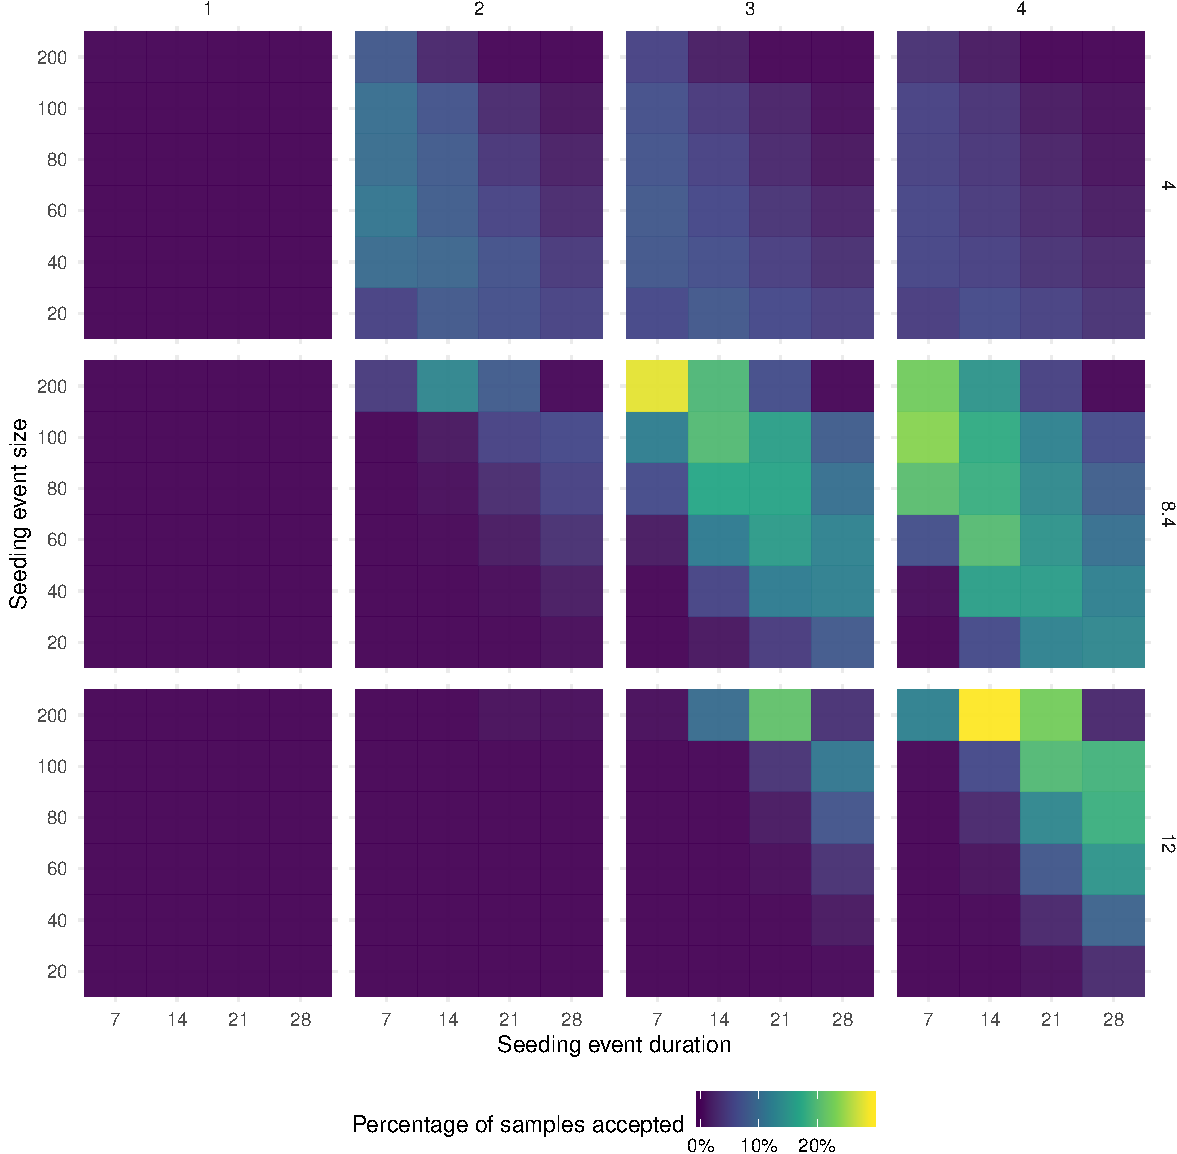
\includegraphics{figures/plot-probs-1.pdf}
\caption{Heatmaps of the percentage of samples accepted by scenario. The
figure is stratified by the upper bound on the reproduction number
(columns) and the mean of the serial interval (rows).}
\end{figure}

\textbf{Estimated reproduction number}

The estimated reproduction number decreased as the event size and
duration increased for both mean serial interval scenarios (Table 1 and
Table 2). Assuming a longer serial interval (12 days) resulted in an
approximate increase of 1 to the reproduction number estimates across
all scenarios when compared to the SARs like (8.4 days) serial interval.
For the SARs like interval the most likely scenario - with an event size
of 200 and a duration of a week) (Figure 1) resulted in an estimated
reproduction number of 2.4 (1.6 - 3.9) (Table 1). Decreasing the event
size increased the reproduction number to 3.1 (2 - 4) for a seeding
event with 100 cases. A longer seeding event resulted in a decrease in
the reproduction to 2.6 (1.6 - 4). The most likely scenario with a mean
serial interval of 12 days - with an outbreak size of 200 and a duration
of 14 days - resulted in an estimated reproduction of 3.3 (2 - 4) (Table
2). For the longer mean serial interval assumption (12 days) varying the
seeding event size and duration had a similar impact on estimates of the
reproduction number. The majority of scenarios had upper bounds
constrained by our assumption of the maximum reproduction number of this
outbreak being 4.

\begin{longtable}[]{@{}lllll@{}}
\caption{Median, minimum, and maximum reproduction numbers of the Wuhan
outbreak conditioned on case data from the 3rd, 18th and 25th of January
- for scenarios with a mean serial interval of 8.4 (SARs like).
Stratified by initial seeding event size and duration.}\tabularnewline
\toprule
Seeding event size vs.~Seeding event duration & 7 & 14 & 21 &
28\tabularnewline
\midrule
\endfirsthead
\toprule
Seeding event size vs.~Seeding event duration & 7 & 14 & 21 &
28\tabularnewline
\midrule
\endhead
20 & 3.8 (3.1 - 4) & 3.5 (2.4 - 4) & 3.3 (1.8 - 4) & 3 (1.7 -
4)\tabularnewline
40 & 3.6 (2.9 - 4) & 3.4 (1.9 - 4) & 2.9 (1.7 - 4) & 2.6 (1.6 -
4)\tabularnewline
60 & 3.5 (2.3 - 4) & 3.1 (1.9 - 4) & 2.6 (1.7 - 4) & 2.3 (1.5 -
3.9)\tabularnewline
80 & 3.3 (2.1 - 4) & 2.8 (1.8 - 4) & 2.4 (1.5 - 3.7) & 2.2 (1.4 -
3.2)\tabularnewline
100 & 3.1 (2 - 4) & 2.6 (1.6 - 4) & 2.3 (1.5 - 3.4) & 2 (1.4 -
3.4)\tabularnewline
200 & 2.4 (1.6 - 3.9) & 2 (1.4 - 3.1) & 1.8 (1.3 - 2.5) & 1.7 (1.5 -
1.9)\tabularnewline
\bottomrule
\end{longtable}

\begin{longtable}[]{@{}lllll@{}}
\caption{Median, minimum, and maximum reproduction numbers of the Wuhan
outbreak conditioned on case data from the 3rd, 18th and 25th of January
- for scenarios with a mean serial interval of 12. Stratified by initial
seeding event size and duration.}\tabularnewline
\toprule
Seeding event size vs.~Seeding event duration & 7 & 14 & 21 &
28\tabularnewline
\midrule
\endfirsthead
\toprule
Seeding event size vs.~Seeding event duration & 7 & 14 & 21 &
28\tabularnewline
\midrule
\endhead
20 & - & 3.7 (3.7 - 3.7) & 3.8 (3.2 - 4) & 3.7 (2.2 - 4)\tabularnewline
40 & - & 3.9 (3.6 - 4) & 3.7 (2.9 - 4) & 3.6 (2.3 - 4)\tabularnewline
60 & - & 3.8 (3 - 4) & 3.7 (2.5 - 4) & 3.4 (2.1 - 4)\tabularnewline
80 & 3.9 (3.9 - 3.9) & 3.8 (2.9 - 4) & 3.6 (2.3 - 4) & 3.3 (2 -
4)\tabularnewline
100 & 3.9 (3.8 - 4) & 3.7 (2.7 - 4) & 3.5 (2.2 - 4) & 3.1 (1.8 -
4)\tabularnewline
200 & 3.7 (2.7 - 4) & 3.3 (2 - 4) & 2.7 (1.7 - 4) & 2.4 (1.6 -
3.9)\tabularnewline
\bottomrule
\end{longtable}

\hypertarget{discussion}{%
\subsection{Discussion}\label{discussion}}

In this study we explored a range of scenarios for the initial event
size and duration of the animal-to-human crossover event which initiated
the 2019-20 Wuhan coronavirus outbreak. We conditioned on observed cases
to establish the probability of each scenario, given our model, and then
estimated the reproduction number of coronavirus virus. We found that
there was a very low probability that the reproduction number was less
than 1 for any scenario considered. For scenarios with a SARs like
serial interval, large seeding events over a short duration were most
plausible. For scenarios with a longer serial interval (12 days), large
seeding events with a slightly increased duration were most plausible.
The most probable SARs like serial interval scenarios resulted in an
estimated reproduction number of 2.4 (1.6 - 3.9), whilst the most
probable longer serial interval scenarios resulted in an estimated
reproduction number of 3.3 (2 - 4). Reducing the event size led to
estimates of the reproduction number increasing but also reduced the
proportion of samples accepted. Similarly, increasing the event duration
reduced the estimated reproduction number whilst decreasing the
proportion of accepted samples.

Our study used a stochastic model to capture the transmission dynamics
of the outbreak with parameters informed from data were possible or
assumed to be similar to those estimated for SARs {[}4{]}. As the
outbreak progresses direct simulation may become too computationally
demanding to be practical so other approaches may be required. More data
is likely to become available, in particular disease specific estimates
for the serial interval, during the course of the outbreak. This will
make it possible to estimate the reproduction number with greater
precision with less risk of bias due to unknown paramters. The number of
scenarios that need to be evaluated will also be reduced as additional
information about cases connected to the initial animal-to-human
crossover event becomes available. Though our estimates had wide
credible intervals it is possible that we could not fully account for
the numerous sources of bias and uncertainty present in the available
data. This means that our model estimates may be both spuriously precise
and potentially biased. However, until more is known about the outbreak
this cannot be easily assessed. However, we made use of a highly
reproducible framework (an R package) and have released all of our code
as open-source. This means that this analysis may be repeated - both by
the authors and others - as more data becomes available. In addition,
subject area experts may be able to adapt our analysis using this
open-source code to reduce the potential for bias using their expert
knowledge.

As the outbreak progress more data will become available on the number
of cases, and the duration of the serial interval. These data are likely
to improve our estimates of the reproduction number and also alter the
likelihood of certain scenarios. Additional data may also lead to a
reevaluation of the suitability of the negative binomial distribution
for generating new cases - or at least provide an outbreak specific
estimate of the dispersion. Our analysis did not include interventions,
such as case isolation, doing so may improve our estimates. The R
package we have developed alongside our analysis may be generalisable to
other point source outbreaks. Additional work is needed to ensure the
robustness of this tool but this may allow this analysis to be repeated
during future outbreaks with little additional overhead.

This analysis use a stochastic branching process to explore scenarios
around the duration and size of the initial animal-to-human crossover
event at the Huanan seafood wholesale market in Wuhan. Despite the
scarcity of data currently available our estimates may be used to rule
out some scenarios and to assess the likelihood of others. Our results
indicate that it is very unlikely that the infectious agent responsible
for the Wuhan outbreak has a reproduction number of less than 1, unless
the size of the seeding event was much greater than currently reported.
As more information becomes available it may also be possible to further
refine our results and establish the reproduction number of the outbreak
more firmly. Providing clear quantitive information for decision makers
on the transmissibility of the infectious agent is of clear public
health importance during outbreaks. Our work to make this process
reproducible may reduce the time these estimates take to be made
available in future outbreaks.

\textbf{Contributors}

All authors conceived and designed the work. SA undertook the analysis
with advice from all other authors. SF developed the branching process
model. SA wrote the first draft of the paper and all authors contributed
to subsequent drafts. \emph{placeholder} reviewed the analysis code. All
authors approve the work for publication and agree to be accountable for
the work.

\textbf{Funding}

\emph{Need funding statement}

\textbf{Competing interests}

There are no competing interests.

\textbf{Accessibility of data and programming code}

The code for this analysis, interim results, and final results can be
found at: \emph{need zenodo DOI link}

\hypertarget{references}{%
\subsection{References}\label{references}}

\hypertarget{refs}{}
\leavevmode\hypertarget{ref-Imai:webreport}{}%
1 Imai N, Dorigatti I, Cori A \emph{et al.} \textbf{Report 2: Estimating
the potential total number of novel Coronavirus cases in Wuhan City,
China}.
\url{https://www.imperial.ac.uk/media/imperial-college/medicine/sph/ide/gida-fellowships/2019-nCoV-outbreak-report-22-01-2020.pdf}

\leavevmode\hypertarget{ref-Thompson:2020bc}{}%
2 Thompson RN. 2019-20 Wuhan coronavirus outbreak: Intense surveillance
is vital for preventing sustained transmission in new locations.
\emph{bioRxiv} 2020;1--14.

\leavevmode\hypertarget{ref-bbc:wuhan:report}{}%
3 \textbf{China coronavirus 'spreads before symptoms show'}.
\url{https://www.bbc.co.uk/news/world-asia-china-51254523}

\leavevmode\hypertarget{ref-Lipsitch:2003}{}%
4 Lipsitch M. Transmission Dynamics and Control of Severe Acute
Respiratory Syndrome. \emph{Science} 2003;\textbf{300}:1966--70.

\leavevmode\hypertarget{ref-R}{}%
5 R Core Team. \emph{R: A language and environment for statistical
computing}. Vienna, Austria:: R Foundation for Statistical Computing
2019. \url{https://www.R-project.org/}

\leavevmode\hypertarget{ref-bpmodels}{}%
6 Funk S. \emph{Bpmodels: Analysing chain statistics using branching
process models}. 2020. \url{https://github.com/sbfnk/bpmodels}

\leavevmode\hypertarget{ref-Boettiger:2015dw}{}%
7 Boettiger C. An introduction to Docker for reproducible research.
\emph{ACM SIGOPS Operating Systems Review} 2015;\textbf{49}:71--9.

\end{document}
